\section{Introduction}
%%%%%%%%%%%% MID WAY AGENDA %%%%%%%%%%%%%%
\begin{frame}{Introduction}{da Vinci robot}<beamer>
\begin{itemize}
\item Minimally invasive surgery, faster recovery
%Minimally invasive surgery is becoming more and more common in hospitals. These procedures are performed through tiny incisions instead of one large opening, requiring a high degree of accuracy.
\item Surgical robots teleoperated by specially trained surgeon through console

\item 3D visual feedback received by surgeon
\end{itemize}

\begin{textblock*}{0.7\textwidth}(4.5cm,3.5cm) % {block width} (coords)
	\begin{figure}[H]
		\centering
		\centering
		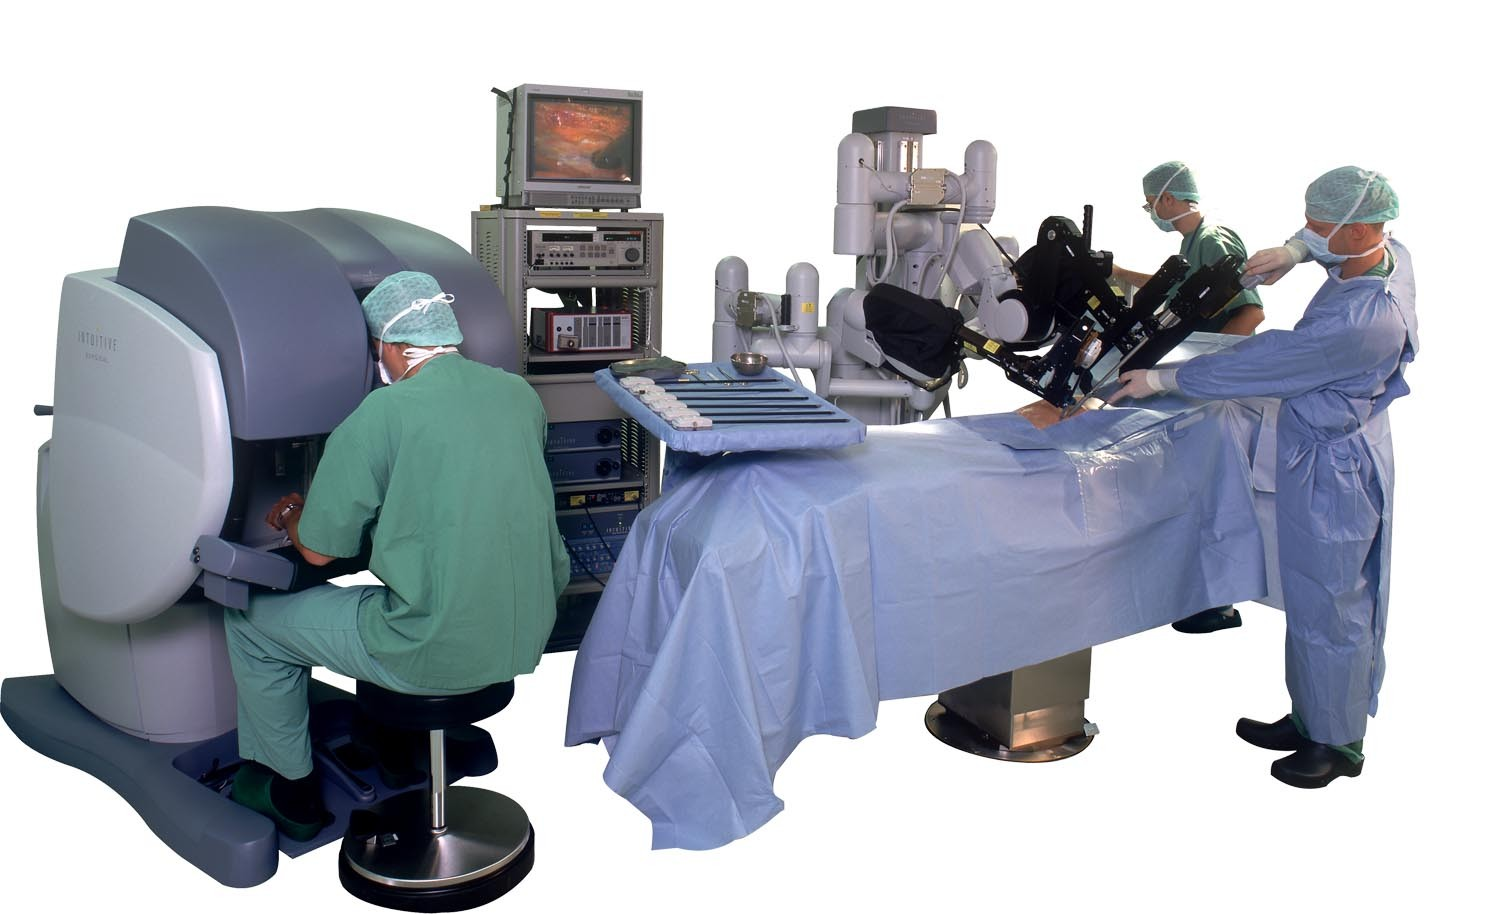
\includegraphics[width=1\textwidth]{Billeder/Dan/davinci.jpg}
	\end{figure}
\end{textblock*}

\end{frame}

\begin{frame}{Introduction}{Limitations of the da Vinci}<beamer>
\begin{itemize}
\item Surgeon has to estimate the force exerted by the tool
\item Studies show haptic feedback reduces error rate
\end{itemize}

\begin{textblock*}{0.7\textwidth}(4.5cm,3.5cm) % {block width} (coords)
  \begin{figure}[H]
  	\centering
  		\centering
  		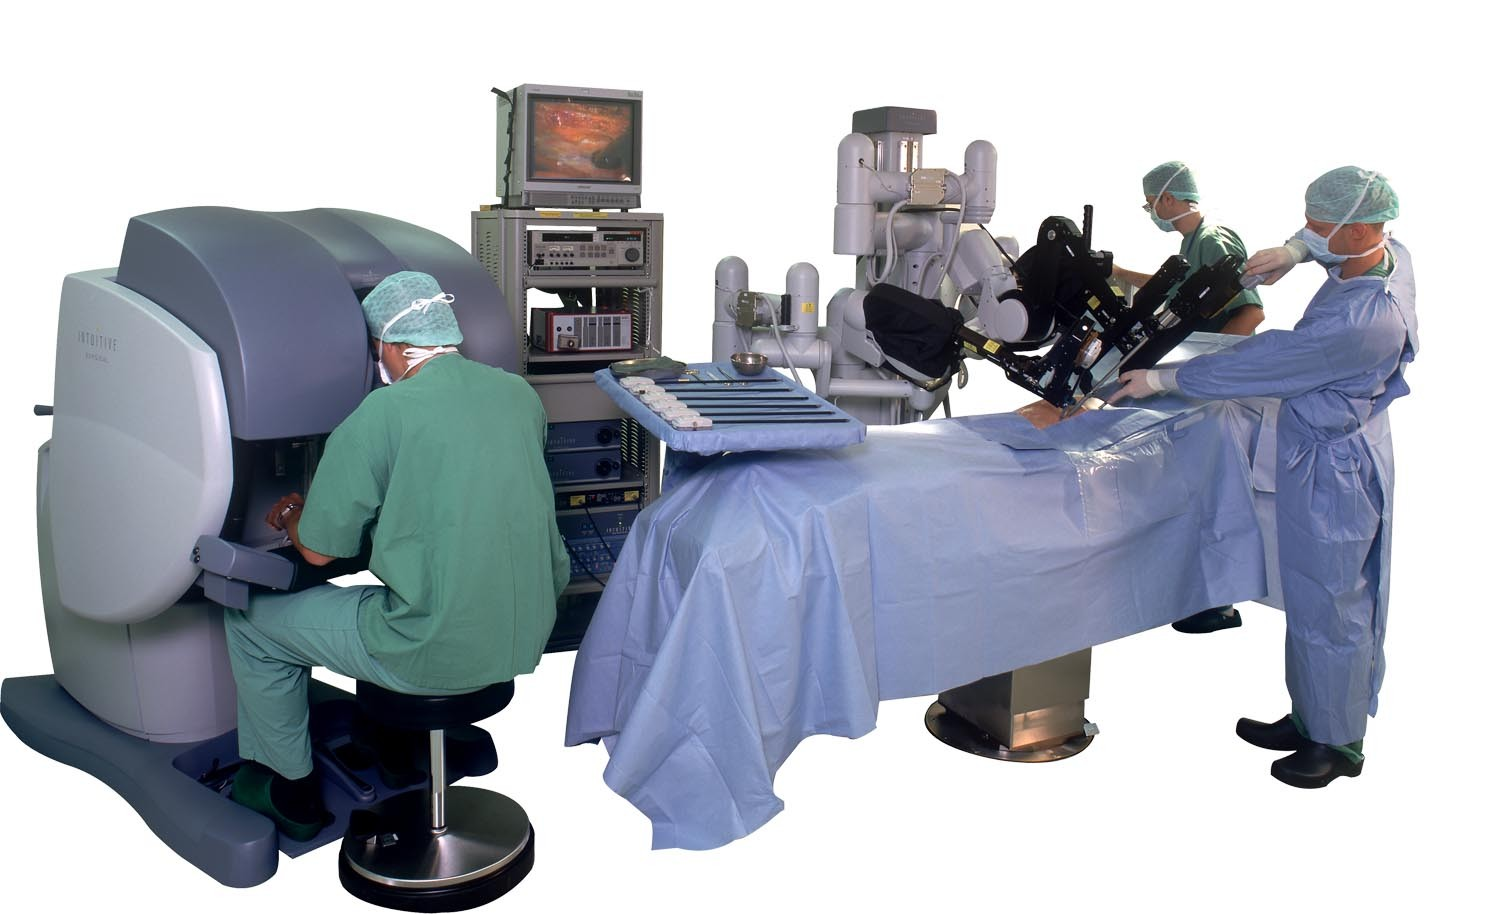
\includegraphics[width=1\textwidth]{Billeder/Dan/davinci.jpg}
  \end{figure}
\end{textblock*}

\end{frame}

\begin{frame}{Introduction}{Test setup}<beamer>
\begin{itemize}
\item Force feedback teleoperation of surgical tool
\item Geomagic Touch 
\begin{itemize}
\item 3 actuated degrees of freedom 
\item Cartesian force feedback
\item Outputs up to 3 N of force
\end{itemize}
\item EndoWrist
\begin{itemize}
	\item No force sensor
	\item High temperature sterilization
	\item Discarded after a couple of uses
\end{itemize}
\end{itemize}

\begin{figure}
	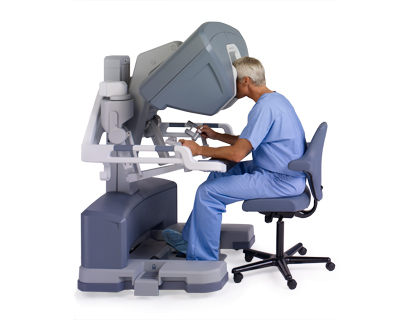
\includegraphics[width=0.3\textwidth]{Billeder/Dan/console.jpg}
	%\hspace{8mm}\vspace{-8mm} $\Rightarrow $ \vspace{8mm}\hspace{8mm}
	\resizebox{0.1\textwidth}{0.05\textwidth}{$\Rightarrow $}
	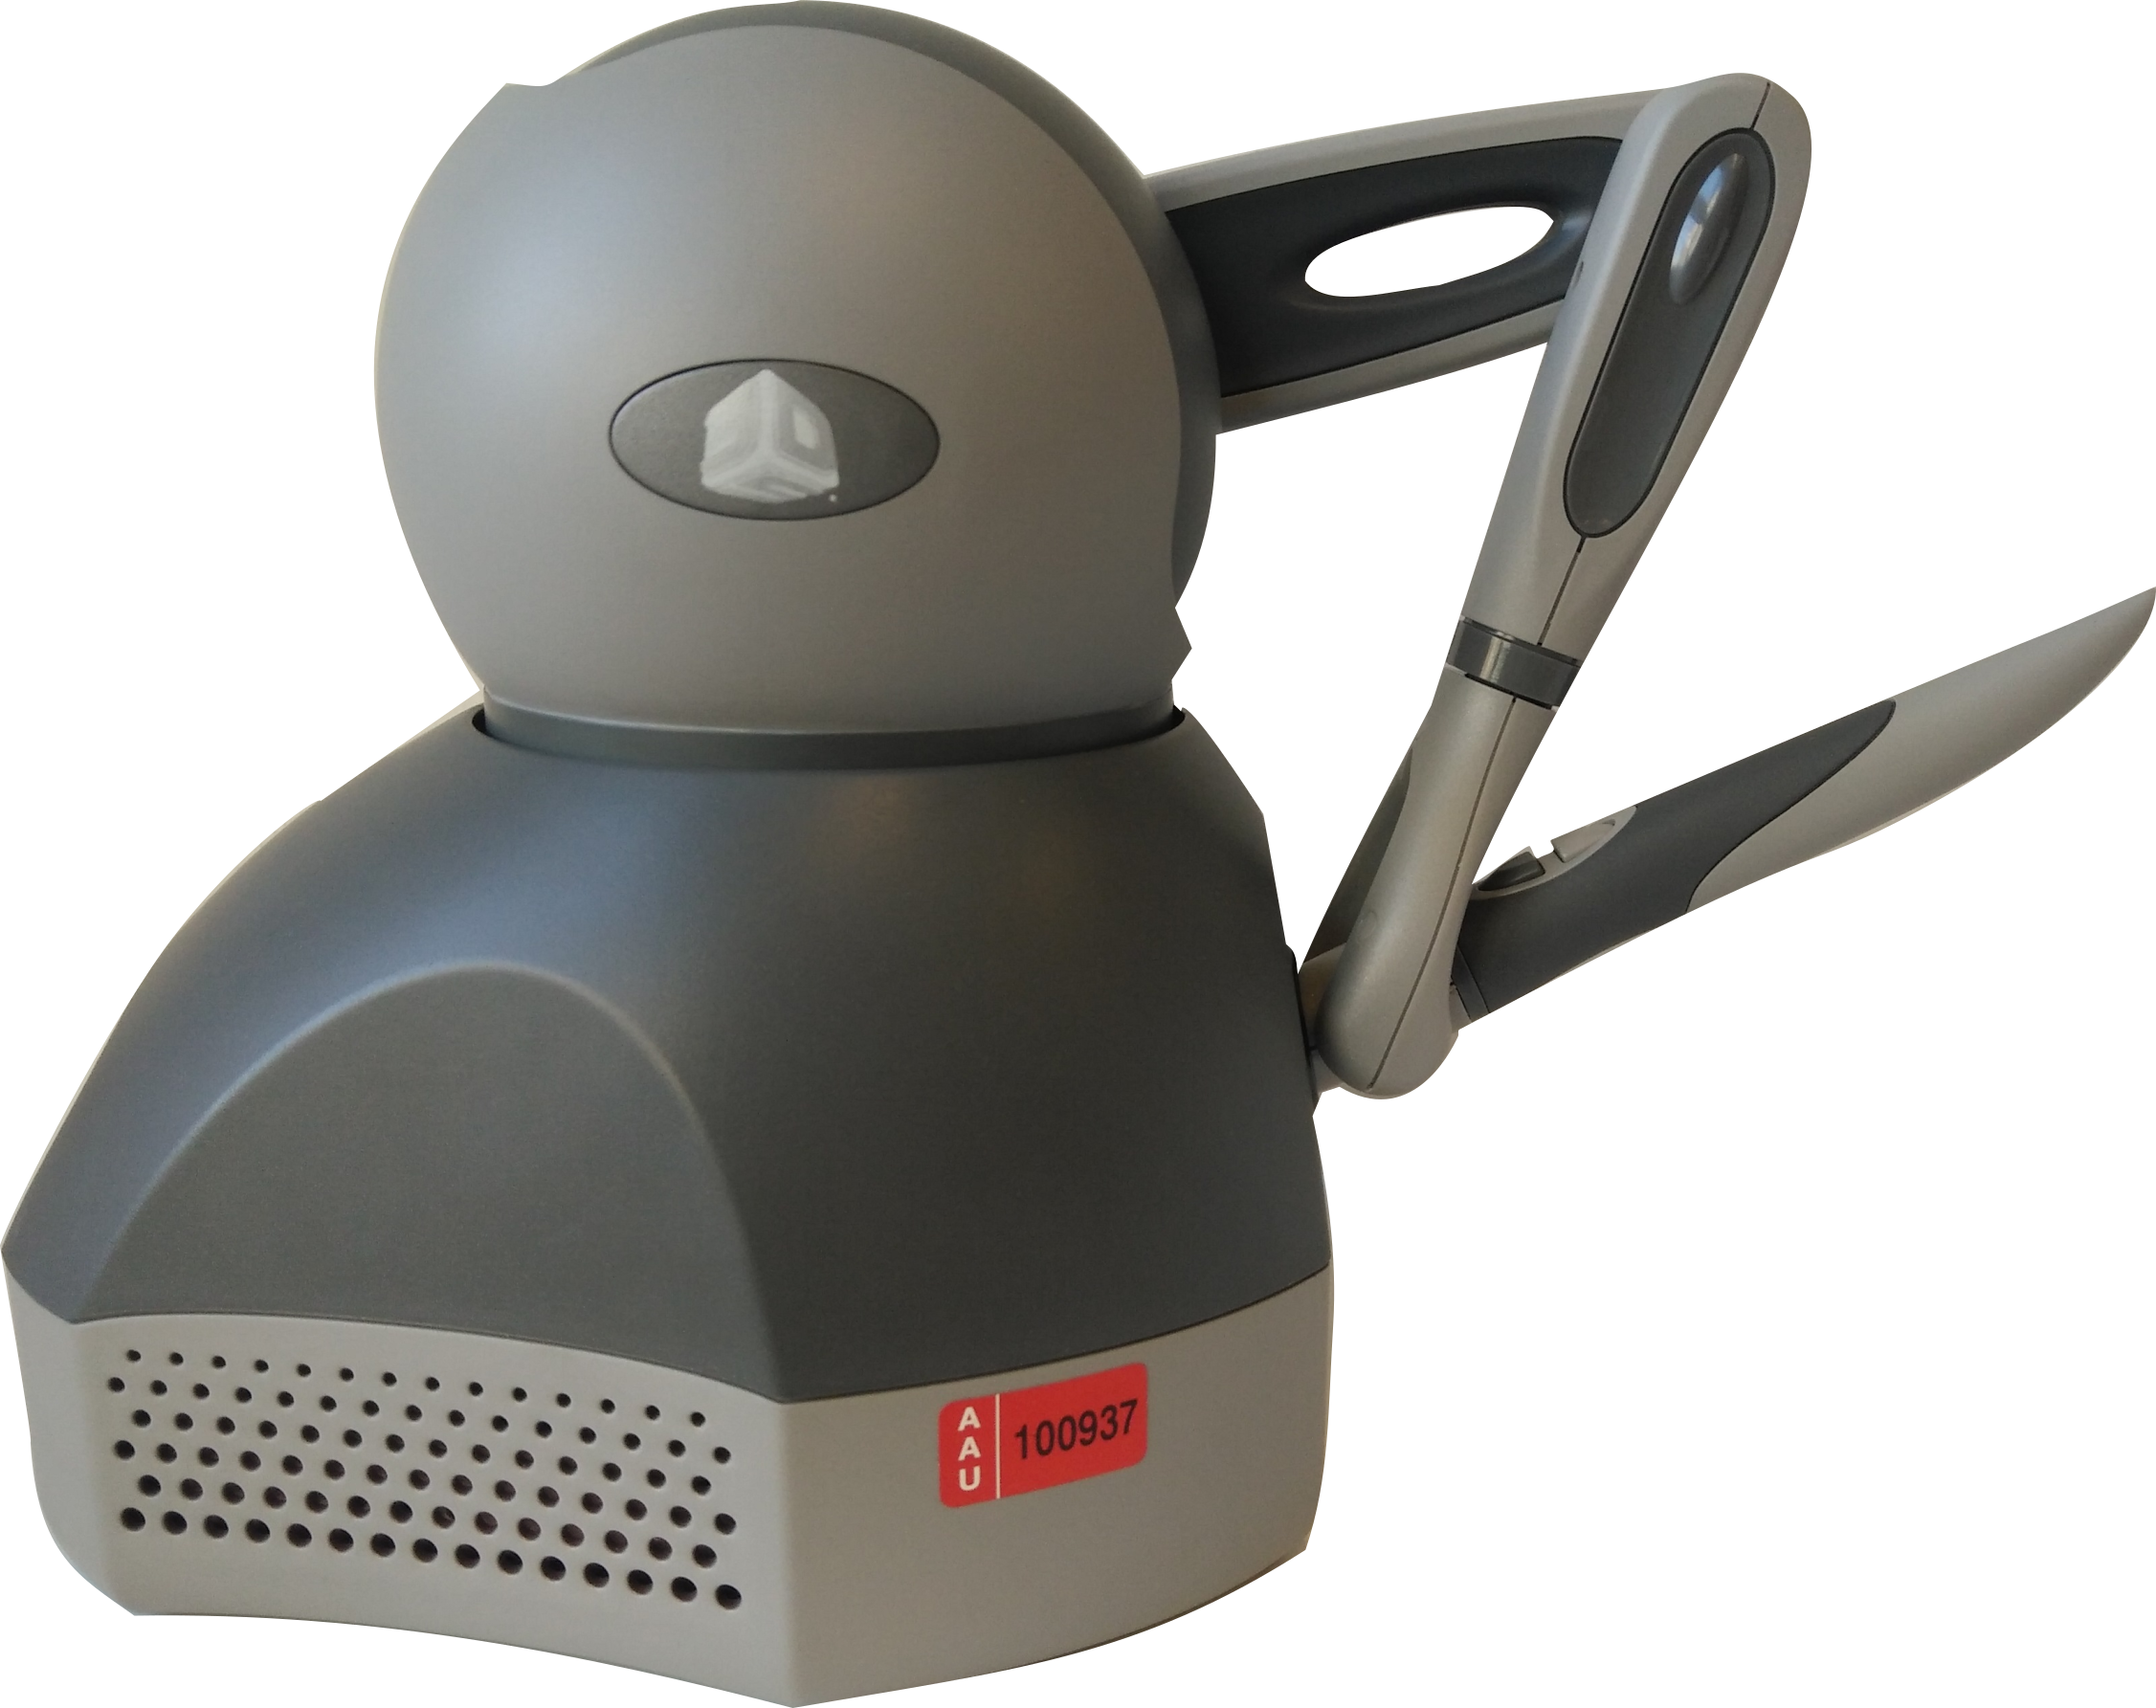
\includegraphics[width=0.3\textwidth]{Billeder/GT.png}
\end{figure}

\begin{textblock*}{0.7\textwidth}(8cm,3.5cm) % {block width} (coords)
	\begin{figure}[H]
		\centering
		\centering
		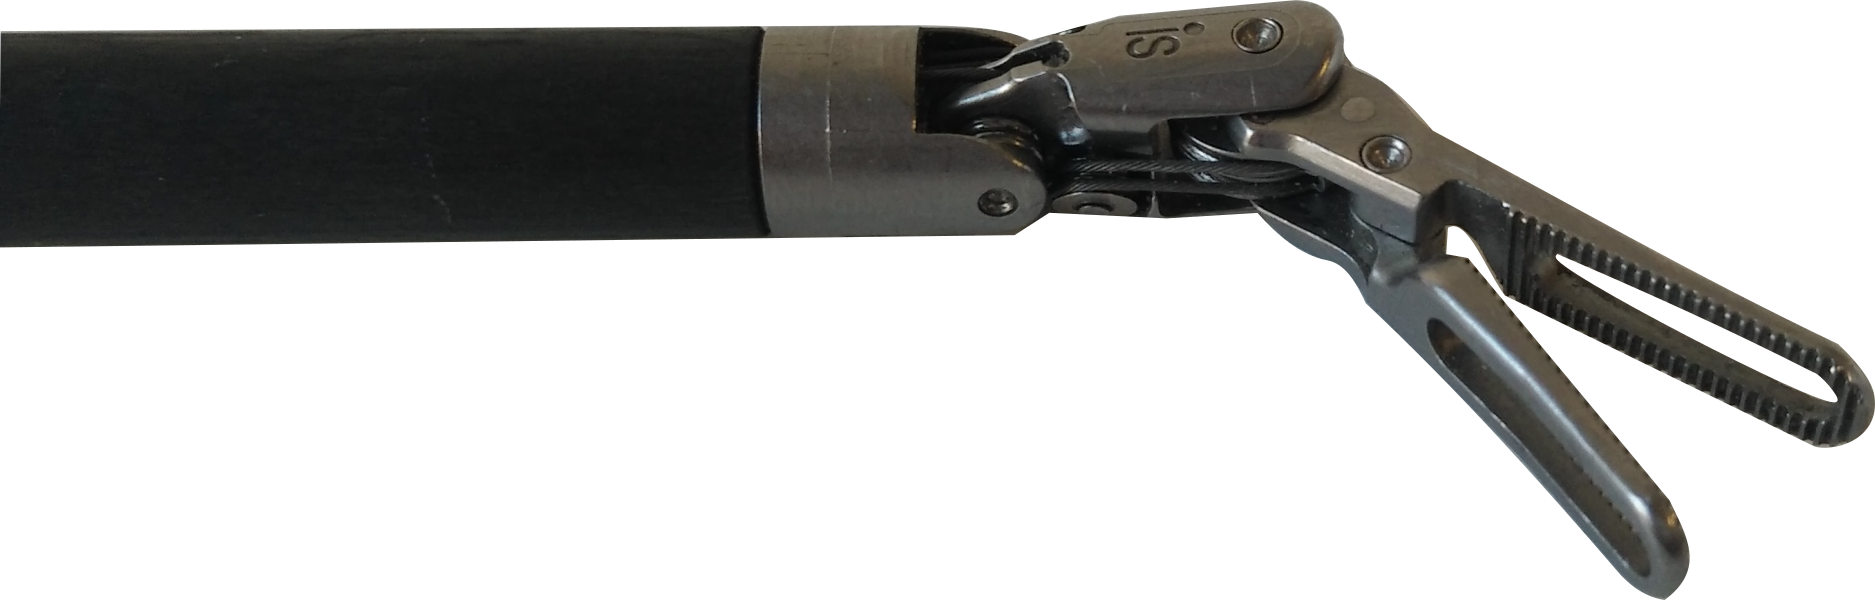
\includegraphics[width=0.4\textwidth]{Billeder/endo2.png}
	\end{figure}
\end{textblock*}


\end{frame}

\begin{frame}{Introduction}{Problem formulation}<beamer>
\begin{itemize}
\item Communication
\begin{itemize}
\item Minimize delays in communication
\end{itemize}
\item Force estimation
\begin{itemize}
\item Sensors too expensive for short lifetime of tools, EndoWrist dynamics have to be modelled
\end{itemize}
\item Control
\begin{itemize}
\item Remove oscillations in force feedback
\end{itemize}
\end{itemize}
\end{frame}